% !TEX root = ../main.tex
%-------------------------------------------------------------------------------
\section{Empirical data}\label{Empirical data}
%-------------------------------------------------------------------------------
We use the same data as in \citet{Keane.1997}. Please see \url{https://bit.ly/ekw-data} for details.

\subsection{Model fit}

We provide a full stack of comparisons between simulated and empirical data. We simulate a sample of 1,000 individuals using the calibrated model.

\begin{figure}[h]\centering
	\caption{Model fit I}\label{Model fit I}
	\subfloat[Blue-collar]{\scalebox{0.19}{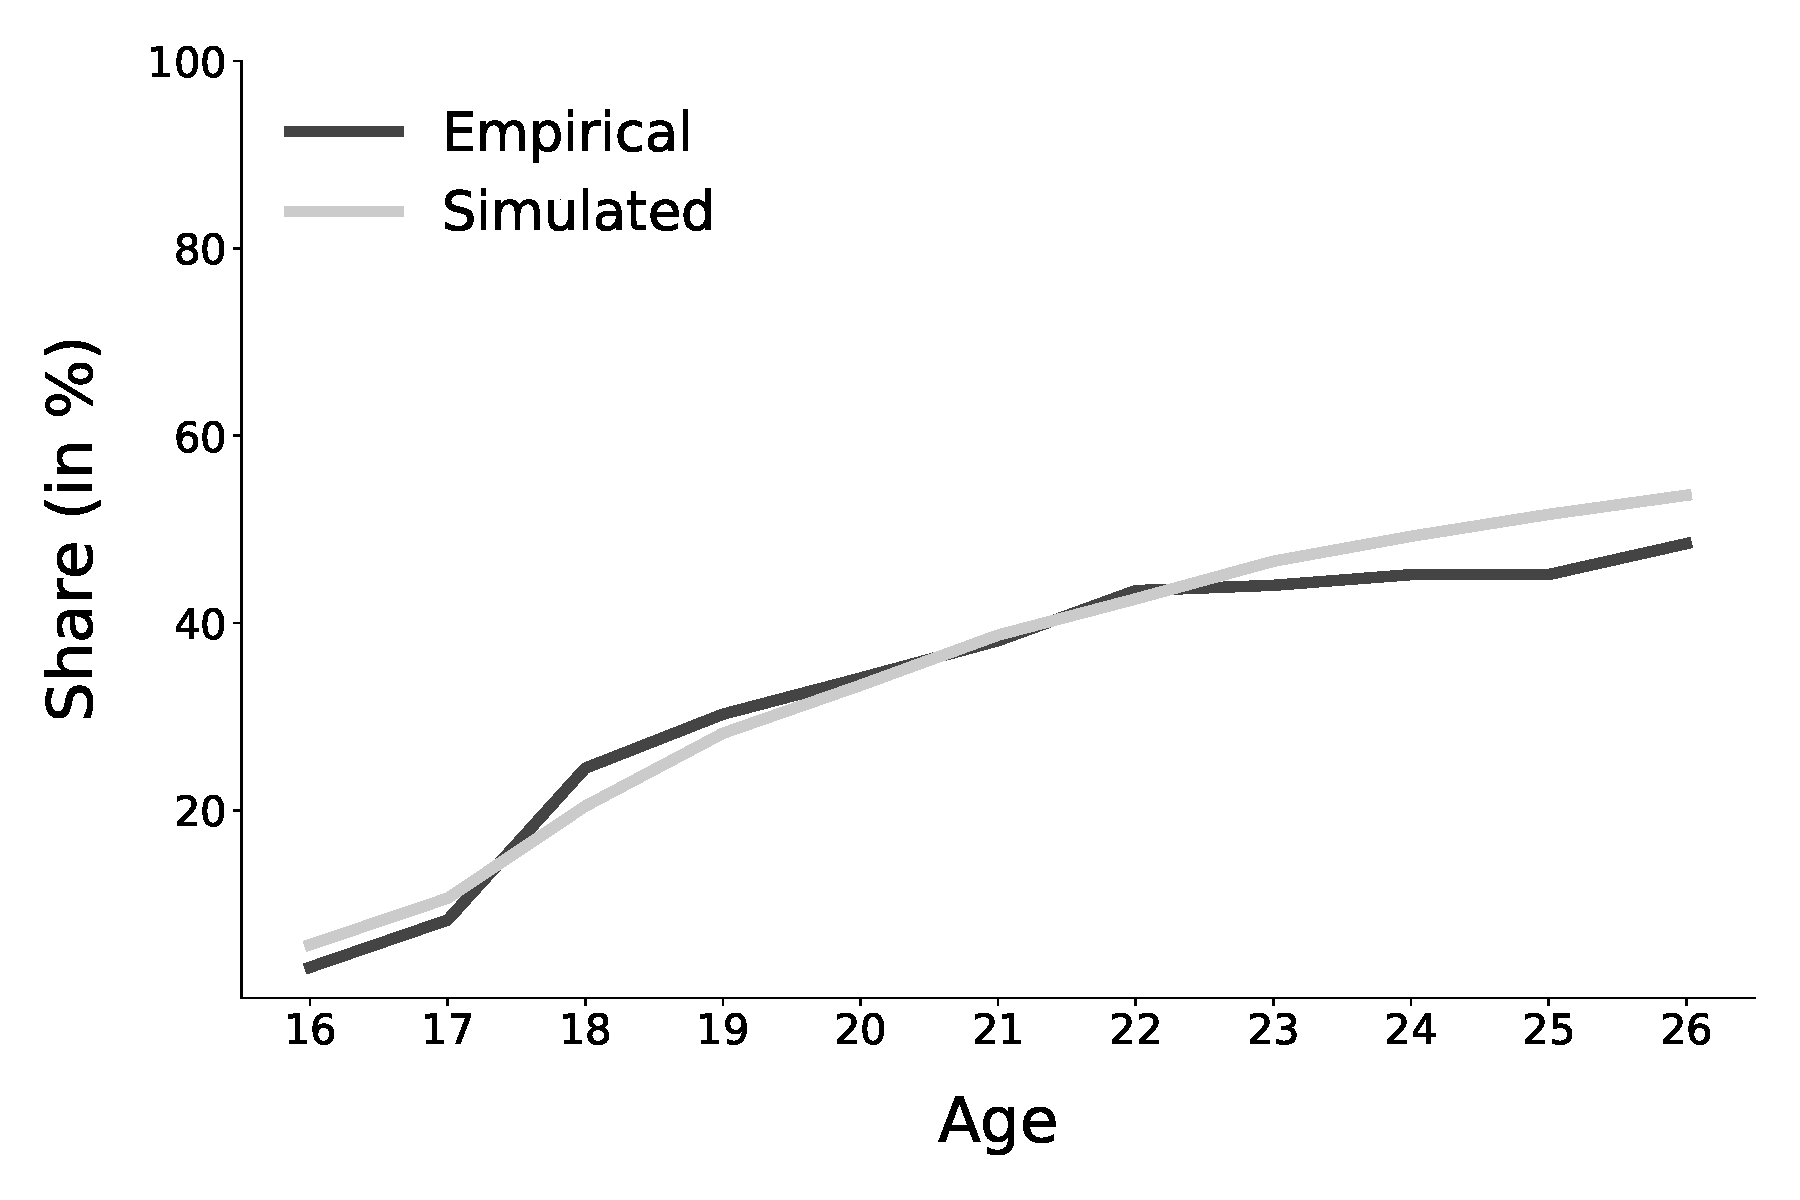
\includegraphics{fig-model-fit-choice-blue-bw}}}\hspace{0.3cm}
	\subfloat[Average wage]{\scalebox{0.19}{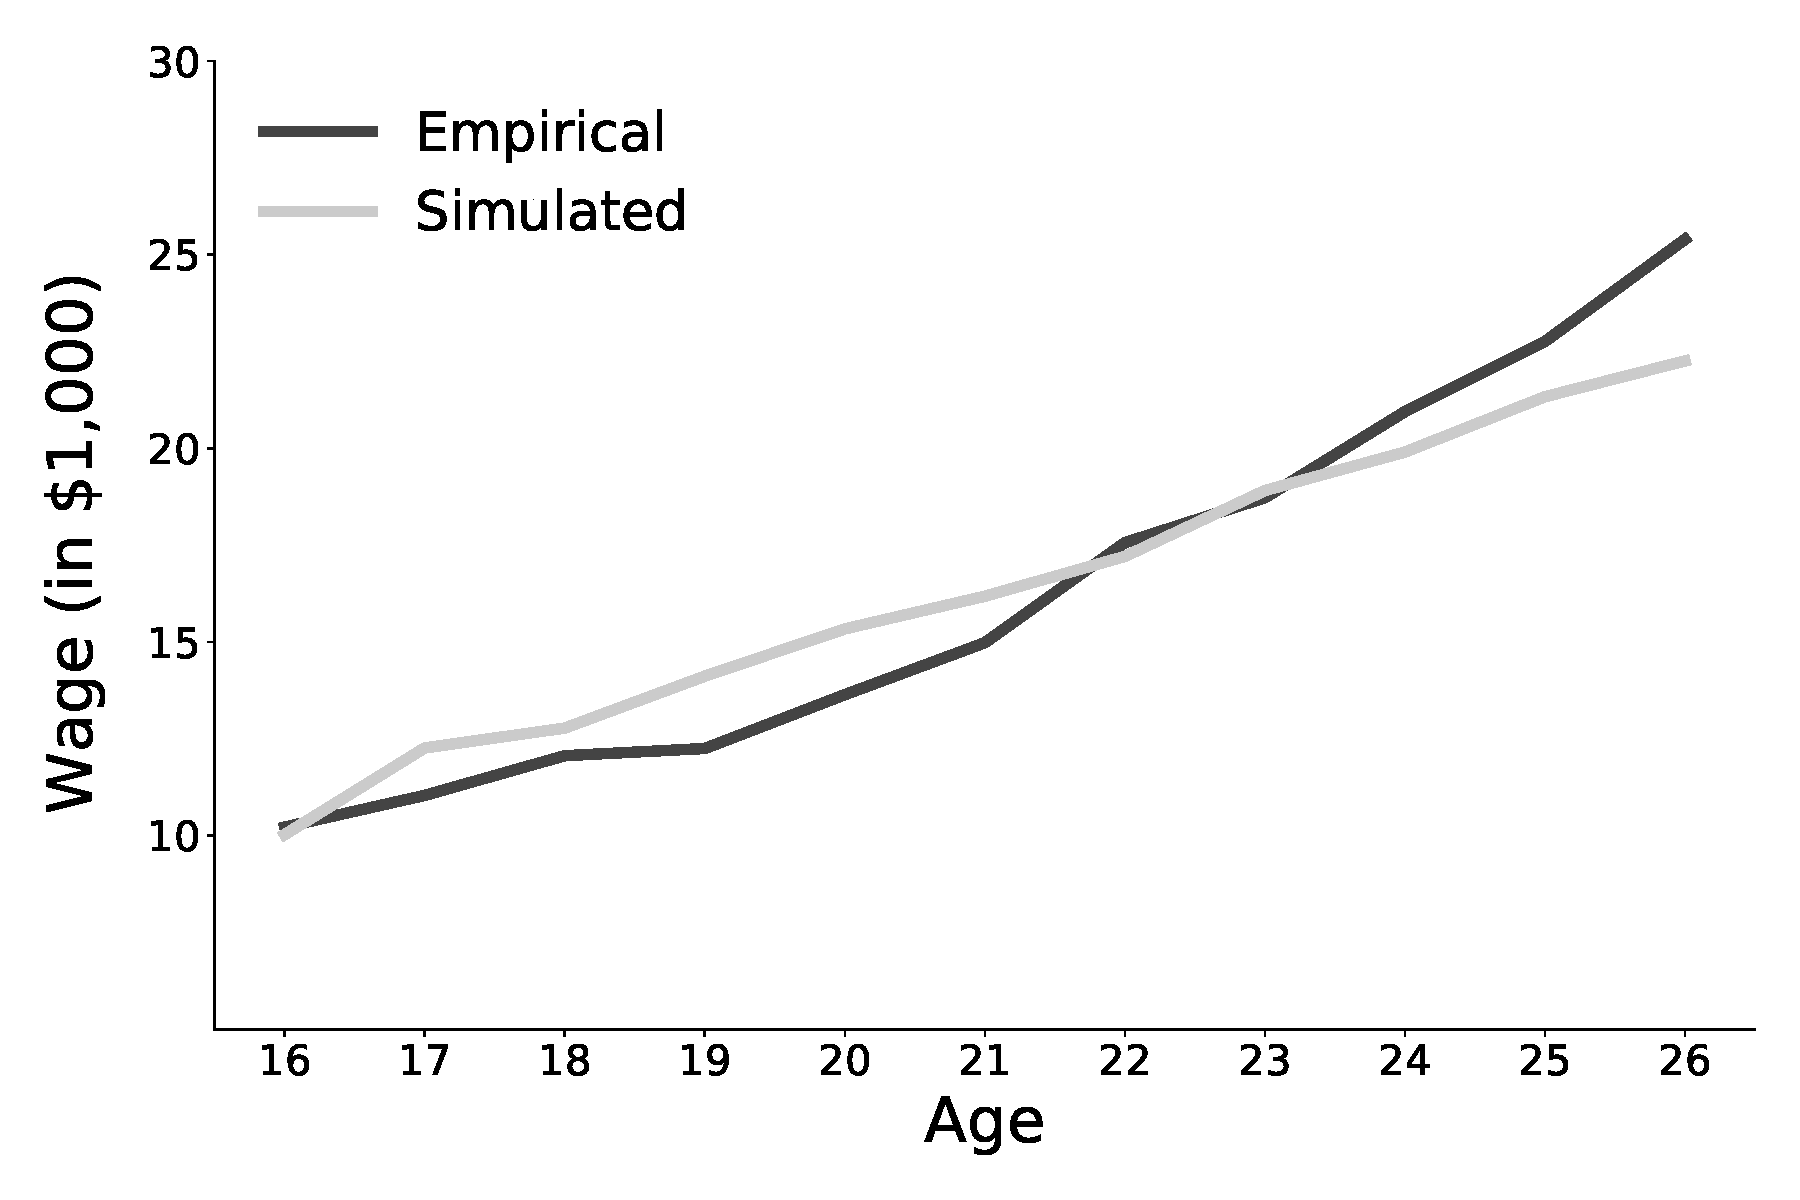
\includegraphics{fig-model-fit-wage-all-bw}}}
	\begin{center}
\end{center}
\end{figure}

\begin{figure}[h]\centering
	\caption{Model fit II}\label{Model fit II}
	\subfloat[White-collar]{\scalebox{0.19}{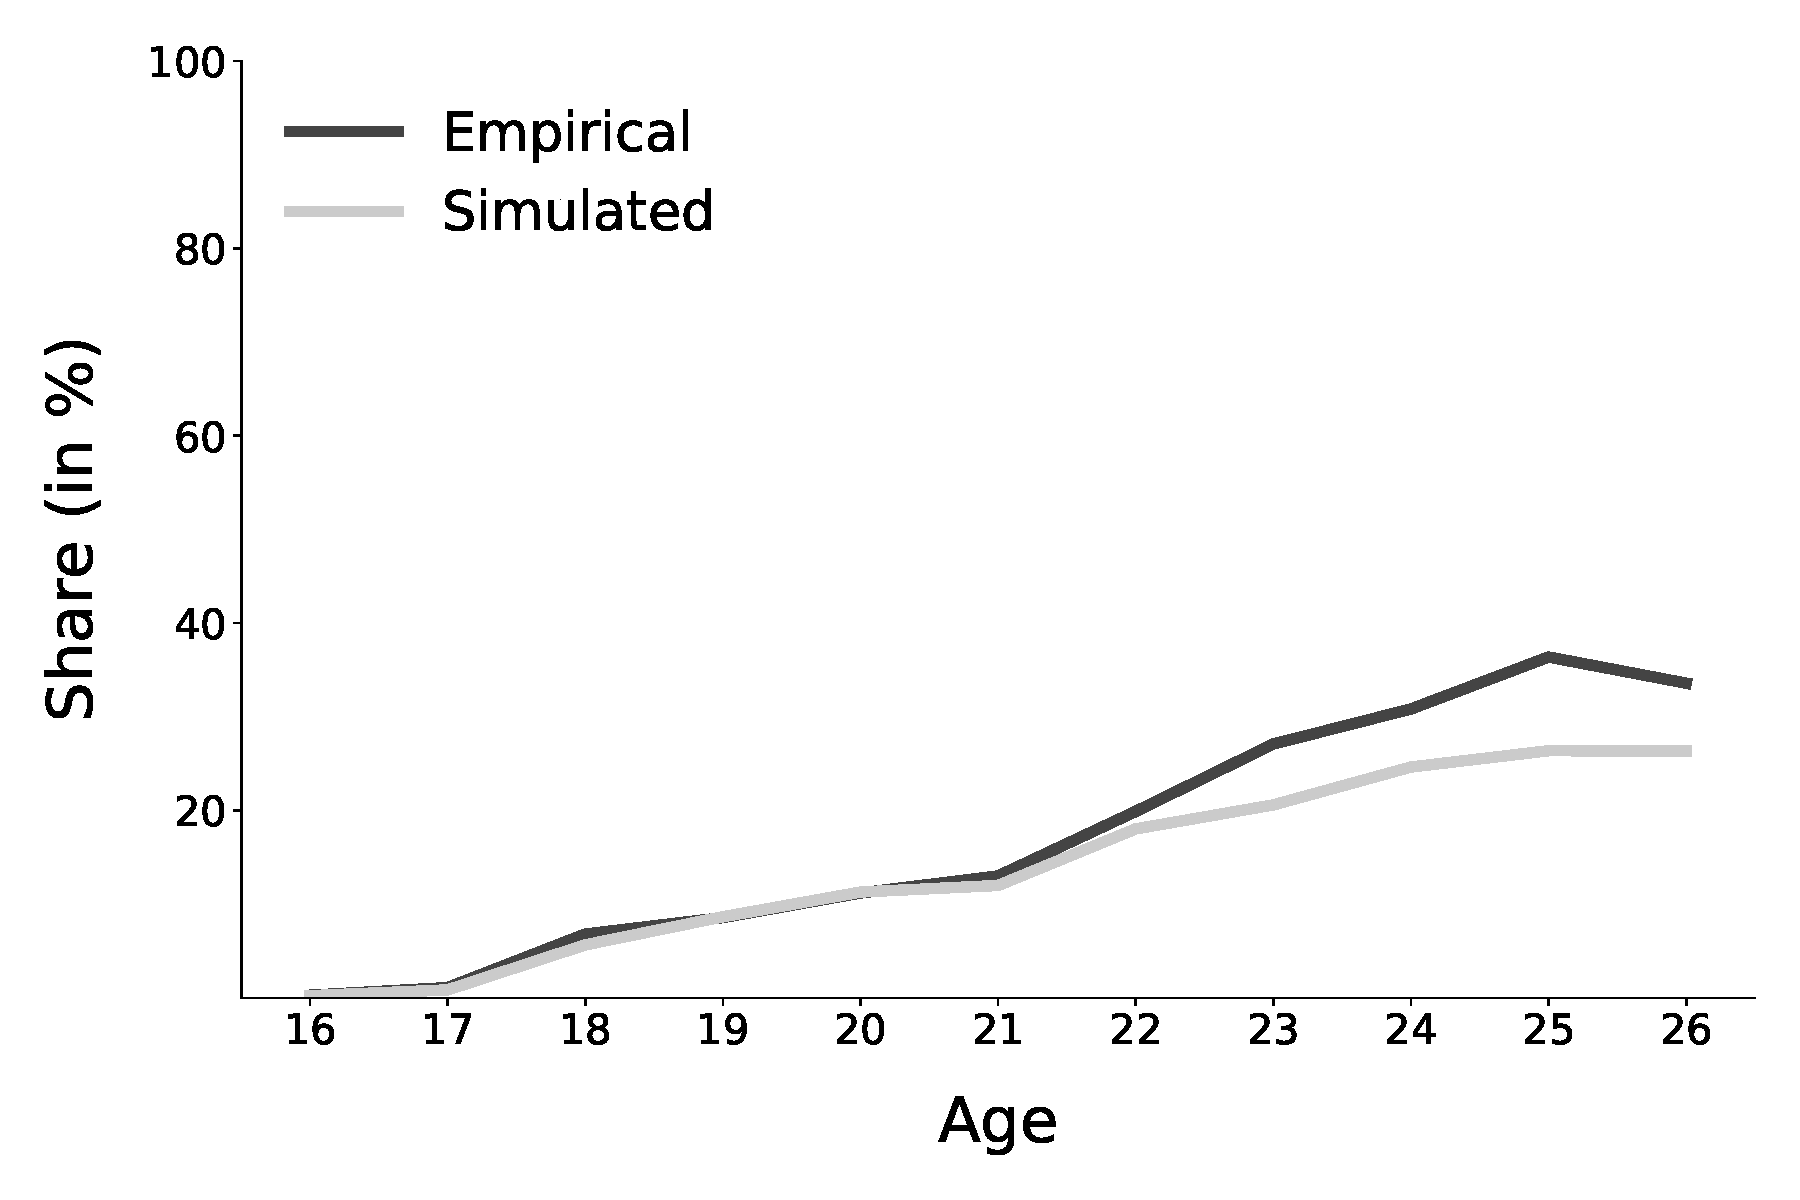
\includegraphics{fig-model-fit-choice-white-bw}}}\hspace{0.3cm}
	\subfloat[Military]{\scalebox{0.19}{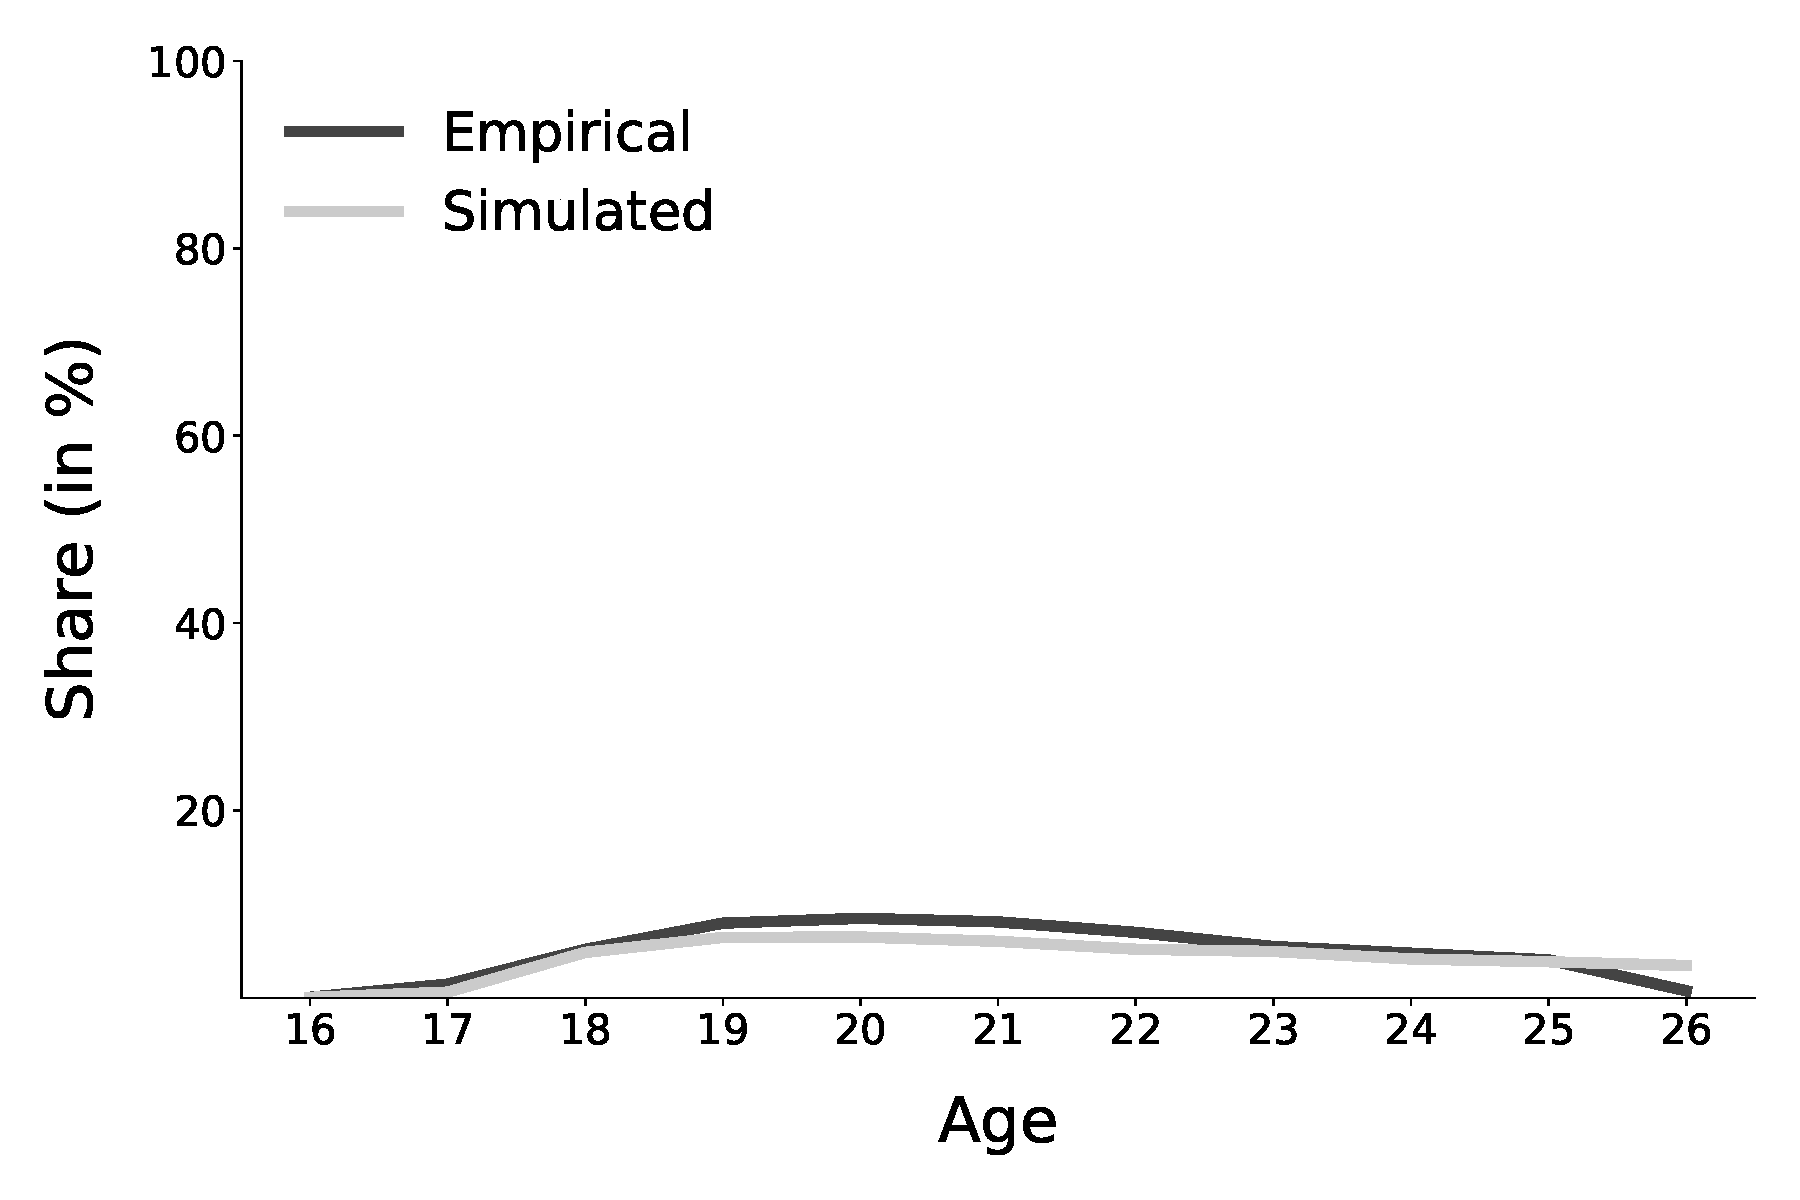
\includegraphics{fig-model-fit-choice-military-bw}}}
	\begin{center}
\end{center}
\end{figure}

\begin{figure}[h]\centering
	\caption{Model fit III}\label{Model fit III}
	\subfloat[School]{\scalebox{0.19}{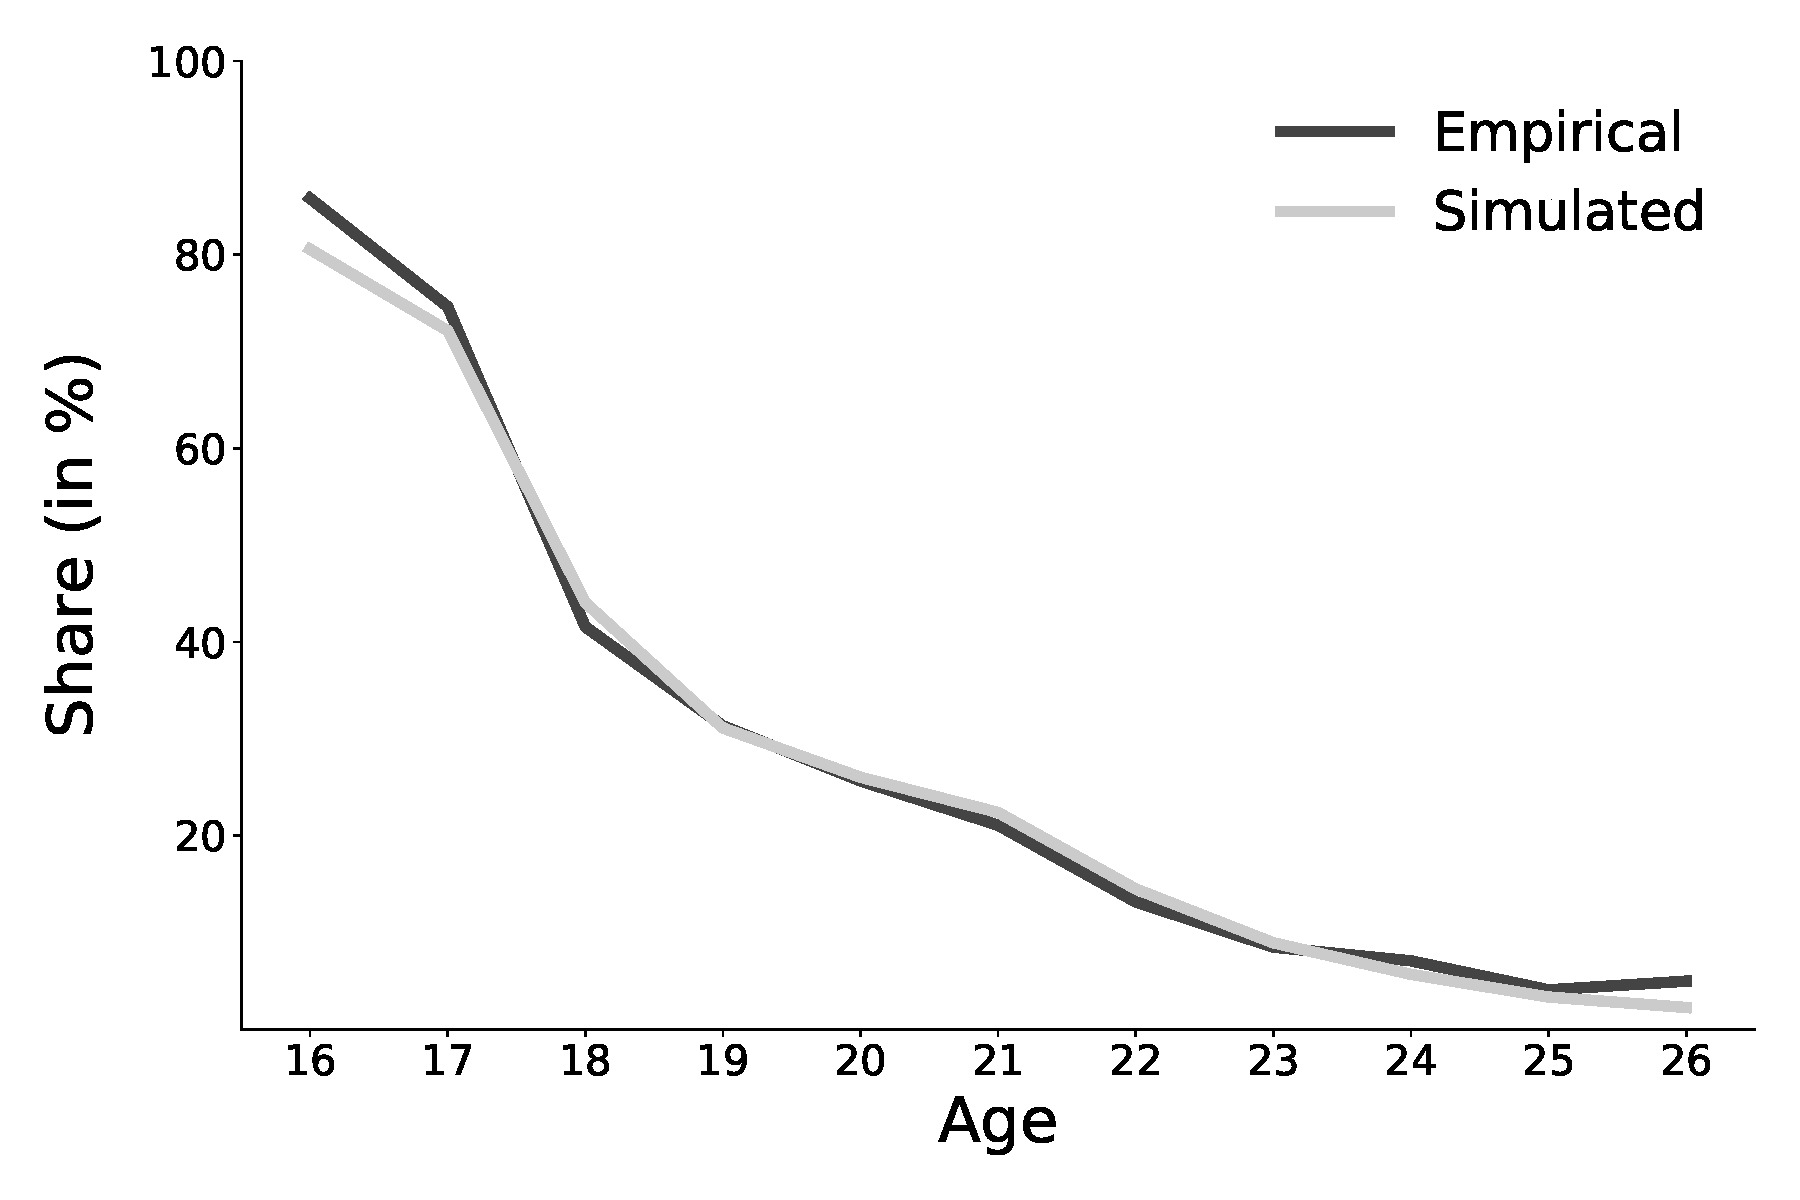
\includegraphics{fig-model-fit-choice-school-bw}}}\hspace{0.3cm}
	\subfloat[Home]{\scalebox{0.19}{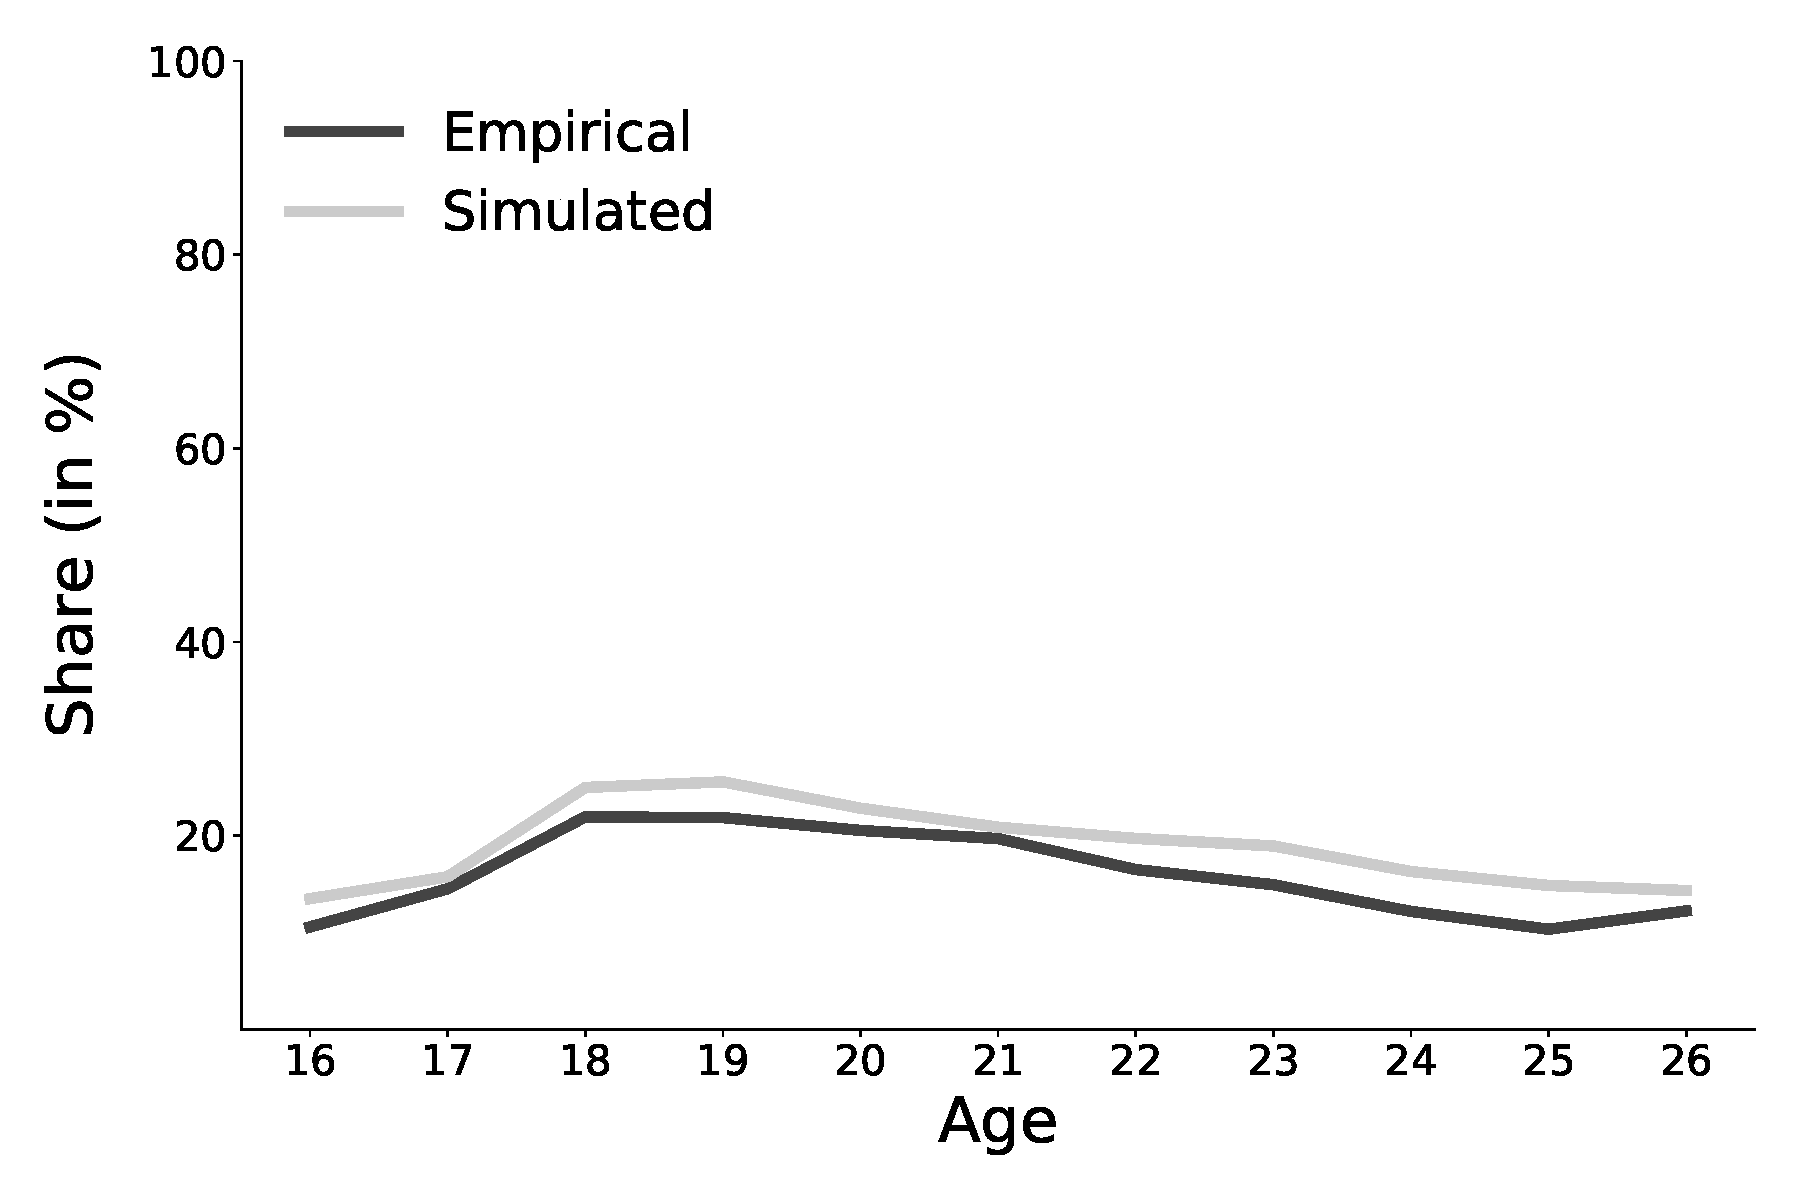
\includegraphics{fig-model-fit-choice-home-bw}}}
	\begin{center}
\end{center}
\end{figure}